% !TeX program = pdflatex
%=======================================================================
% paper.tex -- JMLR submission source.
%
% Standalone paper in the official jmlr2e style, with its own bibliography
% and TikZ schematics. Its numbered statements are self-contained: Hypothesis H,
% Definitions 1-4, Lemmas 1-3, Proposition 4 and Theorem 5.
%
% chktex-file 1
% chktex-file 2
% chktex-file 3
% chktex-file 8
% chktex-file 12
% chktex-file 13
% chktex-file 24
% chktex-file 25
% chktex-file 44
% Compilation is checked separately; these are intentional math and JMLR forms.
% Build:  latexmk -pdf -bibtex paper.tex (or ./scripts/build.sh slim)
%=======================================================================

\documentclass[twoside,11pt]{article}

\usepackage{styles/jmlr2e}
\usepackage{amsmath}
% The array package supports the verification table and must be loaded here:
% without it, this toolchain's epstopdf-base takes the branch that requires
% grfext.sty, which a minimal TinyTeX does not ship, and the build stops with
% "File `grfext.sty' not found".
\usepackage{array}
\usepackage{tikz}
\usetikzlibrary{arrows.meta,calc,positioning}
% Preserve the JMLR geometry without vertically stretching short pages.
\raggedbottom
% Long commit hashes and command paths need emergency stretch rather than
% protruding into the margin.
\setlength{\emergencystretch}{3em}

% The paper's definitions have their own counter (Definition 1..4), while
% lemma/proposition/theorem share one, reproducing Lemma 1, Lemma 2,
% Lemma 3, Proposition 4, Theorem 5.
\newtheorem{defn}{Definition}

% Two unnumbered named environments (Hypothesis H; Proposition [Mask
% Criterion]), defined by hand so that amsthm is not needed and the
% official .sty stays untouched.
\makeatletter
\newenvironment{hyp}[1][]{\par\medskip\noindent\textbf{Hypothesis\ifx\relax#1\relax\else\ #1\fi:}\ \itshape}{\par\medskip} % chktex 6
\newenvironment{uprop}[1][]{\par\medskip\noindent\textbf{Proposition\ifx\relax#1\relax\else\ (#1)\fi:}\ \itshape}{\par\medskip} % chktex 6
\makeatother

\newcommand{\argument}{\par\medskip\noindent\textbf{Argument.}\ }
\newcommand{\qedbox}{\hfill$\blacksquare$}
\newcommand{\ev}{\mathrm{ev}}
% Underscore of a Lean declaration name with a line break allowed after it.
\newcommand{\ttu}{\textunderscore\allowbreak}

\jmlrheading{}{}{}{11/26}{}{}{Shuo Zhang, Yiping Zeng, Shengfeng Luo, and Haichuan Zhang}
\ShortHeadings{A Conditional Risk Gap for Frozen Context Rules}{Zhang, Zeng, Luo, and Zhang}
\firstpageno{1}

\hypersetup{hidelinks,
  pdftitle={A Conditional Risk-Gap Bound for Frozen Context Rules in Open Inversion Tasks},
  pdfauthor={Shuo Zhang, Yiping Zeng, Shengfeng Luo, and Haichuan Zhang},
  pdfsubject={Open inversion tasks; conditional risk gap; provenance; frozen context rules; inverse problems},
  pdfkeywords={open inversion tasks, conditional risk gap, provenance, frozen context rules, inverse problems}}

% Pins the trailer /ID so that the build is byte-reproducible (build.sh
% fixes CreationDate/ModDate through SOURCE_DATE_EPOCH).
\ifdefined\pdftrailerid % chktex 1
  \pdftrailerid{C0FFEE0123456789ABCDEF0123456789}% synthetic constant, not a real identifier
\fi

\begin{document}

\title{A Conditional Risk-Gap Bound for Frozen Context Rules in Open Inversion Tasks}

\author{\name Shuo Zhang \email aki.petit@icloud.com \\ % chktex 1
       \name Yiping Zeng \email zengyiping@sztu.edu.cn \\
       \name Shengfeng Luo \email luoshengfeng@sztu.edu.cn \\
       \name Haichuan Zhang \email zhanghaichuan@sztu.edu.cn\thanks{Corresponding author.} \\[2pt]
       \addr Shenzhen Technology University\\ % chktex 1
       3002 Lantian Road, Pingshan District\\
       Shenzhen, Guangdong, China 518118}

\editor{Action Editor}

\maketitle

\begin{abstract}%
Frozen context rules---parameters fixed before inference---are often treated as general-purpose solvers for inverse problems whose observations are ill-posed and whose test inputs leave the training distribution. We distinguish evidence- or analytic-instantiated rules (Mode~A) from offline-frozen rules (Mode~B) by the provenance of their values, and ask when a specified class of frozen rules can be uniformly accurate. Under a bounded-description condition, a demand barrier, and a scale-restricted realization condition, we prove a positive risk gap; whenever it is positive, no rule in the class is uniformly accurate at any smaller tolerance. A minimal instance shows that the assumptions are jointly satisfiable, and an edge-aware denoising interpretation connects the bound to a concrete inverse problem. The result limits solo completeness, not the usefulness of frozen components in composite systems.
\end{abstract}

\begin{keywords}
  open inversion tasks, conditional risk gap, provenance, frozen context rules, inverse problems
\end{keywords}

\section{Introduction}
\label{ch:intro}%

Many inference tasks are ill-posed. For example, monocular 3D reconstruction seeks the surface depth associated with each image pixel, but pixel brightness admits infinitely many depths; likewise, a measurement can admit infinitely many states, and no local observation alone fixes the answer \citep{hadamard1902}. Ill-posedness can arise from the observation model itself: projection, sampling, and noise can remove information about the underlying structure. Early vision stated this systematically, with stereo vision, motion estimation, optical flow, and shape reconstruction admitting a unique solution only after additional constraints \citep{poggio1985}. Contextual constraints restrict the degrees of freedom left undetermined by local observations; examples include neighboring pixels on one surface and frames on one motion.

The required contextual constraints are generally spatially and temporally heterogeneous: strong inside a surface, so that the neighborhood corroborates and noise is smoothed away; cut at boundaries and occlusions, so that the two sides form independently, else depth smears along edges. How strongly context should be used therefore varies with position and time, its correct value depending on where the scene's boundaries lie and where motion breaks: a context rule is a stipulation varying with the evidence, not a fixed law.

\subsection{Open Inversion Tasks}

Three items delimit the base class: (P1) observations are ill-posed, (P2) the required context strength is heterogeneous and content-addressed by the evidence, and (P3) inference inputs may come from outside the training distribution---the \emph{open set}. A task satisfying P1--P3 is an \emph{open inversion task}. The impossibility results use a fourth, separately stated hypothesis: (P4) relative to a specified comparison class, the required context rule cannot be given within every pre-given tolerance on the open set by values frozen before inference begins. Real-time 3D reconstruction motivates these criteria \citep{kerbl2023}, as do image and video restoration, online state estimation, and medical and scientific inversion; membership in the base class and satisfaction of P4 must be checked separately for each concrete task.

These items are premises whose failure delimits the conclusion: a homogeneous interpolation task fails P2; in fixed-grid simulation the boundary positions are set by the task rather than the evidence; under fixed operating conditions the demand is exogenous; and a demand exactly identifiable from a fixed corpus fails P4. Frozen context-rule components on such tasks are outside what the conditional result excludes. In particular, no motivating example is asserted to satisfy P4 without a separate argument.

\subsection{The Solo-Completeness Hypothesis}

We study a deliberately strong working hypothesis, not a claim that we attribute to a specific paper. Universal approximation and scaling results motivate the view that a single sufficiently trained component might remove the need for task-specific adaptation \citep{cybenko1989,hornik1989,bubeck2023,kaplan2020,brown2020}, but none of those works states the hypothesis below; the formalization is ours. Critics who read some emergent abilities as metric artifacts sharpen the need for such a statement rather than settle it \citep{schaeffer2023}.

\begin{hyp}[H]
There exists a frozen context-rule component that, using only that component and without any external proposal or arbitration stage, is complete for open inversion tasks; that is, it solves each task independently across inference distributions and scenarios, without assuming that the test distribution agrees with the training distribution.
\end{hyp}

A \emph{frozen context-rule component} is a component whose context rules are frozen into parameters that do not change at inference time and whose values come from training-corpus statistics or manual setting; neural networks are the canonical instance. Write $\mathcal{H}_{\mathrm{NN}}$ for the specialization of Hypothesis~H to neural-network components. Theorem~5 addresses that specialization only for a specified rule class and under explicit bounded-description and P4 hypotheses. Here \emph{completeness} means independent task solving, not completeness in the sense of mathematical logic. The qualifier ``only'' is crucial: the result does not deny the usefulness of frozen components, including neural feature extractors, within larger systems. High accuracy on a fixed benchmark close to the training distribution is within reach of both kinds of components, but that \emph{weak claim} is not the object here.

The method is conditional deduction, not experimental proof. Hypothesis~H is existential and its negation is a universal statement over a whole task class, so a single counterexample does not settle it. The chain runs from explicitly stated criteria to a capability boundary; experiments can assess those criteria and explore applicability, but cannot validate the universal statement. Accordingly, the paper proves a conditional exclusion for a qualified subclass, not an unconditional real-world negation of H: an application requires a nonvacuous P4/BD instance, a benchmark bound giving $\kappa>0$, and a tolerance below $\kappa$. Lemma~1 holds for a separable data term and an arbitrary even differentiable pairwise potential, with no convexity assumption, but its first-order conditions describe stationary points rather than guaranteed global minimizers in the nonconvex case.

\subsection{Contributions}

The paper makes three contributions.
\begin{enumerate}
\item \emph{A provenance-based decision axis.} Mode~A and Mode~B are defined by where rule-carrying values come from, not by architecture, capacity, or input dependence; Section~\ref{sec:procedure} turns the distinction into an implementation checklist.
\item \emph{A stationarity-ratio obstruction.} If one scalar satisfies the first-order conditions at two positions, their defined stationarity ratios must agree; a frozen position-wise multiplier family is excluded across two configurations exactly when the zero-safe compatibility condition \eqref{eq:tablecondition} fails. The lemma is algebraic: it does not infer a task's demand profile from P2, and objective form alone does not settle provenance.
\item \emph{A conditional risk-gap theorem.} Theorem~\ref{thm:main} gives an explicit barrier, bounded-description, realization, benchmark, and tolerance bound; Section~\ref{sec:instance} supplies a nonvacuous instance; Appendix~\ref{app:proofs} gives complete proofs; and Appendix~\ref{app:verification} separates the algebra and toy closure verified in Lean~4 from the general analytic and modeling premises that are not.
\end{enumerate}

The scope is deliberately narrow. The theorem is not an unconditional statement about all neural networks or all inverse problems, and it does not deny that frozen features, retrieval, or composite systems can be useful. What it identifies is a class-relative boundary: when demand is non-freezable at a realized scale, a specified frozen class cannot achieve uniform accuracy below the gap. Tasks outside P4 or BD are not thereby classified as complete; the theorem is silent about them. This distinction between a scoped negative result and a universal claim is maintained throughout.

\emph{Organization.}
Section~\ref{ch:related} positions the work relative to inverse problems, amortized inference, distribution shift, and retrieval. Section~\ref{ch:formalize} fixes notation and states P1--P4 and assumption A0; Section~\ref{ch:axis} defines the provenance axis. Section~\ref{ch:bound} proves the stationarity-ratio algebra and the conditional risk-gap theorem, and Section~\ref{sec:instance} gives a worked edge-aware instance. Section~\ref{ch:discussion} translates the bound into an evaluation protocol and states limitations. Appendix~\ref{app:proofs} contains complete proofs, and Appendix~\ref{app:verification} documents the Lean artifact.


\section{Related Work}
\label{ch:related}%



The terminology is not cosmetic. ``OOD generalization'' does not imply that observations are ill-posed or that context strength is evidence-addressed; ``frozen model'' does not distinguish a calibration invariant from a corpus statistic; ``model-based'' does not determine whether a fixed analytic map or a learned table supplies the rule; and ``universal approximation'' says nothing about solving a task without the test distribution agreeing with training. The four distinctions are therefore kept separate in the formal development, and the table records the nearest existing concept rather than claiming that no related idea exists.

\emph{Ill-posed inversion and regularization.}
Classical inverse problems characterize ill-posedness through non-uniqueness and unstable dependence on observations \citep{hadamard1902}, and stabilize inversion with Tikhonov regularization, discrepancy principles, L-curves, and generalized cross-validation \citep{tikhonov1977,hansen1992,golub1979}. These methods choose a regularizer and a scalar or spatially varying weight, and establish existence, stability, or data-dependent selection. The question here is different: not how to choose a strength, but whether the provenance of the chosen values permits completeness across an open set. Learned reconstruction makes the distinction concrete: a corpus-trained denoiser, unrolled network, or score-based generative prior is Mode~B \citep{gregor2010,adler2018,ongie2020,song2021}, while a calibration or analytically computed regularizer can be Mode~A. The classification does not deny the in-distribution accuracy of learned reconstruction; it asks what that accuracy implies when the test distribution and the required context change.

\begin{table}[!ht]
\caption{Terminology and the nearest existing concepts. The table states what each term adds; it is not a claim that the existing literature lacks the corresponding phenomena.}
\label{tab:terminology}
\centering
\small
\begin{tabular}{@{}>{\raggedright\arraybackslash}p{0.18\textwidth}>{\raggedright\arraybackslash}p{0.24\textwidth}>{\raggedright\arraybackslash}p{0.50\textwidth}@{}}
\hline
\textbf{Term} & \textbf{Nearest concept} & \textbf{What the term adds}\\
\hline
Open inversion task & Out-of-distribution generalization & P3 is one component; P1 (ill-posedness) and P2 (heterogeneous, evidence-addressed context) are independent requirements.\\
Frozen context-rule component & Frozen or parametric model & The criterion is the provenance of rule-carrying values, not parameter count; an analytic fixed function is Mode~A, a corpus-fitted table is Mode~B.\\
Mode~A / Mode~B & Model-based / data-driven; parametric / nonparametric & Existing labels describe architecture or training; the modes describe where values come from. Equations \eqref{eq:modeA}--\eqref{eq:modeA2} and \eqref{eq:modeB} are behavioral consequences, not definitions.\\
Completeness & Universal approximation; statistical consistency & Independent task solving across inference distributions, not approximation capacity or an asymptotic parameter limit.\\
\hline
\end{tabular}
\end{table}

\emph{Amortized inference and adaptation.}
Variational autoencoders and amortized inference replace per-instance optimization by a learned mapping from observations to approximate posteriors \citep{kingma2014,rezende2014}. The amortization gap measures the additional error of that mapping relative to a per-instance optimum within a variational family \citep{cremer2018}. Our risk gap is not that quantity: it compares a rule's risk with an evidence-instantiated benchmark, not with a per-instance variational optimum, and neither equality nor positivity follows from the analogy. Meta-learning and test-time adaptation make the same point from another direction \citep{finn2017,hospedales2021,sun2020,liang2024}: adapting at inference changes parameters, but it does not by itself change provenance. An analytic per-instance solve is Mode~A; a learned update rule whose values are corpus-fitted remains Mode~B even when it runs online.

\emph{Distribution shift and generalization.}
Domain adaptation theory bounds target risk in terms of source risk, a divergence between domains, and the best joint hypothesis \citep{bendavid2010}; invariant-risk and group-robustness methods add training objectives or regularization for worst-group performance \citep{arjovsky2019,sagawa2020}, and surveys organize the resulting landscape \citep{zhou2022,gulrajani2021,yang2024}. P3 is only one of P1--P3: open inversion adds ill-posed observations and heterogeneous, evidence-addressed context. The theorem is therefore not a general impossibility result for OOD generalization, and it does not claim that domain-generalization methods fail; it constrains a specified frozen class under P4 and BD.

\emph{Approximation and no-free-lunch.}
Universal approximation theorems show that feedforward networks can approximate continuous functions on compact domains \citep{cybenko1989,hornik1989}, with general approximation-theoretic treatments in \citet{pinkus1985}. No-free-lunch theorems show that no algorithm dominates across all problems without a problem-specific prior \citep{wolpert1996,wolpert1997,adam2019}. Our notion of completeness is neither approximation capacity nor algorithm-level universality: it concerns independent task solving across inference distributions, and the bound is relative to a specified provenance class and benchmark. There is no contradiction with approximation theorems, because the target classes, topologies, losses, and hypotheses differ; indeed, the paper states this explicitly after the barrier construction.

\emph{Adaptation, retrieval, and foundation models.}
Large pretrained models adapt to new tasks through prompting, in-context examples, or lightweight updates \citep{brown2020,bommasani2021,kaplan2020}, and test-time adaptation updates parameters from unlabeled inputs \citep{wang2021}. Retrieval augments a frozen model with a nonparametric store \citep{khandelwal2020,borgeaud2022}. These are important escape routes from a purely fixed component, and Hypothesis~H deliberately excludes external proposal or arbitration stages. Our claim is about solo use: adaptation and retrieval can change the system boundary, but they do not by themselves establish that a frozen component is complete without them.

\emph{Uncertainty quantification and calibration.}
Conformal and distribution-free methods provide coverage guarantees under exchangeability or specified distributional assumptions \citep{angelopoulos2021,romano2017}. Those guarantees concern the calibration of a predictor, not the existence of a context rule that remains correct across an open set of tasks. They are complementary: a calibrated component can still be Mode~B, and a Mode~A rule need not be calibrated. The risk gap of Section~\ref{ch:bound} is a statement about rule values, not about predictive intervals.

\emph{External memory, retrieval, and composites.}
Dynamic external memory and retrieval-augmented models extend a network with a store that is read at inference \citep{graves2016,lewis2020,khandelwal2020,borgeaud2022}. Hypothesis~H excludes an external proposal or arbitration stage, not external memory as such; such a component may be paired with retrieval, tools, or a learned controller. The negative result is about solo use within the specified class. Composite systems containing Mode~A are not ruled out, and their system-level completeness requires a separate argument rather than following from the component-level bound.



\section{Formalization of the Problem}
\label{ch:formalize}%

Let the position set $I$ be \emph{finite} throughout---the pixel set in image tasks, or the product of time indices and state components in state estimation---and let the structure field $d : I \to \mathbb{R}$ assign a structure value to every position. Finiteness makes all subsequent sums and squared norms well defined; an infinite-index extension would require a specified summable space. An observation consists of a mask $m : I \to \{0,1\}$ marking the observed positions together with the observed values there: values inside the mask are pinned by the observation, values outside are under no direct constraint.

\begin{defn}
An observation is \emph{ill-posed} if there exist two different structure fields $d \neq e$ that agree with the observed values at every position inside the mask.
\end{defn}

\begin{uprop}[Mask Criterion]
An observation with a hole is ill-posed: if some position $j$ is not covered by the mask, two different values at $j$ give two structure fields compatible with the same observation. Conversely, a mask covering all positions determines the structure field uniquely, so the observation is not ill-posed.
\end{uprop}

Neither direction depends on numerical detail: positions outside the mask are degrees of freedom, two values on one giving a bifurcation, while a full mask pins every position; real observations almost always have holes---depth behind occluding surfaces, bands drowned in noise, null spaces of measurement equations.

\subsection{Criteria for the Base Class and the P4 Subclass}

Criteria P1--P3 define the base class; Criterion P4, together with the explicit implementation hypotheses below, delimits the subclass to which the impossibility result applies. P2 is a task-level modeling criterion, not a premise of Theorem~\ref{thm:main}; it motivates position-dependent strength but does not imply the stationarity-ratio differences in Lemma~1.

\begin{itemize}
\item Criterion P1 (ill-posedness): different structure fields are compatible with the same observation.
\item Criterion P2 (heterogeneity): boundary and interior positions require different consistency strengths, and which is which is content-addressed by the current evidence.
\item Criterion P3 (distributional openness): inputs at inference time are not constrained by the training distribution. The formal results are restricted to mask-modeled inputs satisfying \emph{mask openness}: the observation pins the evidence part while the context part retains uncovered free positions, so the same evidence admits free bifurcation of the context values. This is an additional bridge assumption, not a consequence of distributional openness alone.
\item Criterion P4 (class-relative non-freezability of the demand): relative to a specified comparison class of offline-frozen rules, the demand rule's values cannot be given within every pre-given tolerance on the open set by an object existing before inference begins. Section~\ref{sec:p4} splits the formal hypothesis into a \emph{barrier condition} on the demand and a \emph{scale-restricted realization condition} for a class with a uniform bounded-description rate. These hypotheses yield a positive floor $\kappa$ on the risk gap only when the benchmark bound is small enough.
\end{itemize}

Distributional openness by itself implies neither a mask hole nor P1. Under the separate mask-openness bridge, however, an uncovered position supplies the bifurcation required by P1. The difficulty is thus a progression: ill-posedness forces inference to use context, heterogeneity requires context to vary by position, and openness requires rules to remain correct beyond the training inputs; P4 and BD are additional hypotheses for the quantitative exclusion. A test distribution $P$ is specified for each evaluation: an open set does not mean that no distribution exists, and mask openness is the only form of openness the derivations consume.

\begin{itemize}
\item Assumption A0 (evidence-computability of the demand): The demand rule is computable from current evidence; that is, there exists a mapping from evidence to the values of the demand rule such that on every input the demanded values can be given at inference time by evidence and analytic means.
\end{itemize}

A0 plays no role in the negative risk-gap argument, which instead uses the stated mask, demand, BD, and P4 hypotheses; it supports only the positive, constructive reading of Section~\ref{ch:discussion}. Tasks whose demand depends on unobserved structure with no trace in the evidence fail A0 and remain outside the positive claims. The formal model uses scalar structure fields on $I$; depth, disparity, signed-distance, and vector-valued representations require their own mask models and criterion checks, and no invariance under representation changes is claimed.

\begin{table}[t]
\caption{What each hypothesis supplies and what it does not. The table is a reading guide, not a set of sufficient conditions for one another.}
\label{tab:assumptions}
\centering
\small
\begin{tabular}{@{}>{\raggedright\arraybackslash}p{0.17\textwidth}>{\raggedright\arraybackslash}p{0.30\textwidth}>{\raggedright\arraybackslash}p{0.45\textwidth}@{}}
\hline
\textbf{Object} & \textbf{Supplies} & \textbf{Not implied by}\\
\hline
P1 & An observation with competing structures & A full mask (no hole); a hole is sufficient in the mask model but not necessary.\\
P2 & A demand that varies between boundary and interior and is addressed by evidence & The stationarity-ratio obstruction of Lemma~1.\\
P3 + mask bridge & Test inputs outside the training support, with an uncovered context part & P3 alone; the bridge is separate.\\
P4a & A demand separation $\delta$ at every scale & Any statement about a rule, average, or benchmark.\\
P4b & Positive mass at one class-admissible scale $\eta_*$ & Realization at every scale; that stronger demand is vacuous in the non-atomic model.\\
BD & A uniform rate $\Lambda_0$ for the specified class & Finite description alone; threshold rules can lie outside BD.\\
A0 & Evidence-computable demand for the positive reading & The negative risk-gap argument, which does not use A0.\\
$\mathrm{risk}^*$ & A fixed evidence-instantiated benchmark & A quantity observable from task syntax alone.\\
\hline
\end{tabular}
\end{table}

P4 cannot be read off the task syntax: a task can satisfy P1--P3 and fail P4, and the failure is a modeling judgement about the demand, not a syntactic test. The instance below satisfies P4; no general construction is claimed for tasks that fail it. The barrier condition mentions no rule, average, or benchmark and belongs to the family of classical approximation barriers \citep{kolmogorov1936,pinkus1985}; transmission to a risk gap is a proved inequality under the additional realization and BD hypotheses. Its empirical content sits in the class-relative realization level $p$ and the benchmark risk of the best evidence-instantiated rule, neither of which is assumed to be observable from task syntax alone.

\section{The Decision Axis: Context Rules and Two Modes}
\label{ch:axis}%

Ill-posed tasks cannot do without context, but ``using context'' needs an analyzable handle:

\begin{defn}
A \emph{context rule} is the stipulation of where and how strongly context is needed, and its content is a set of numbers: a family $R = (R_i)_{i \in I}$ of mappings $R_i : (I \to \mathbb{R}) \to \mathbb{R}$, one for each position $i \in I$. Its argument is a \emph{candidate field} $z$: the current numerical hypothesis about the structure, with candidate evidence $z|_{\ev}$ at observed positions and candidate context values elsewhere. A test candidate is also written $d$ when it is the field on which a risk is evaluated. Thus $R_i(z)$ may use both evidence and the candidate's context; a rule that uses context outside $\ev$ is \emph{candidate-adaptive}. The rule is \emph{global} when the family is constant, $R_i = R_j$ for all positions $i, j$, as in the scalar $\lambda$ of classical regularization, and \emph{position-wise} when the family is not constant.
\end{defn}

Structural representations must still be instantiated into numbers wherever they participate in numerical inference. Representation changes the carrier of a rule, not the provenance of its values. The index carries content: Criterion P2 motivates position-dependent strength, with evidence content-addressing boundary and interior. Whether a constant family can nevertheless satisfy the stationarity equations is a separate algebraic question, answered in Lemma~1.

\begin{defn}
A rule belongs to \emph{Mode A} if all content-carrying values are instantiated by current evidence or taken from cross-scenario invariants given by analysis and calibration, such as camera intrinsics. Mode A has two behavioral subcases. \emph{A1 (evidence-only)} uses the candidate only through its evidence. \emph{A2 (candidate-adaptive analytic)} may also use candidate context through an analytic or calibration map, but no content-carrying value is a training-corpus statistic or a manual setting. A rule belongs to \emph{Mode B} if its computation involves content-carrying parameters that are fixed at inference time and whose values come from training-corpus statistics or manual setting. Mode B is disjoint from Mode A by provenance, not by its equations alone. Only parameters that carry the content of the rule participate in the classification. Learning rate, iteration count, step size, and random seed are bookkeeping only when the solver is guaranteed to converge to the same specified unique limit regardless of those choices. For a finite-step computation or a problem with multiple local solutions, they can change the output and therefore participate in the Mode B classification when their values are frozen corpus or manual choices. A component implementing an analytic or calibration function with fixed parameters is Mode A, whereas one implementing a corpus-statistical function remains Mode B even if its output depends only on evidence.
\end{defn}

Pre-existence alone is not the criterion: analytic and calibration invariants may pre-exist inference and remain Mode A. Classification concerns the substantive source of the function and its values, not their storage location, magnitude, or input dependence.

\begin{figure}[t]
\centering
\small
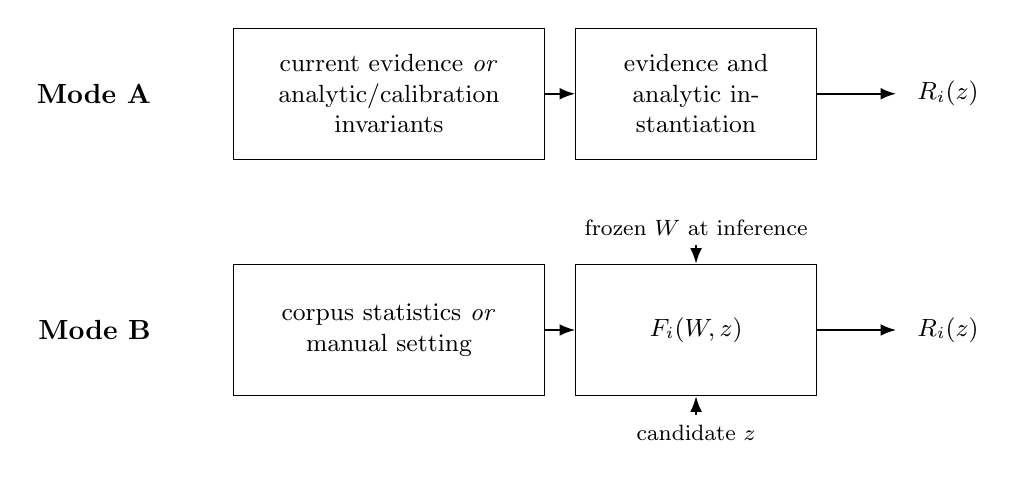
\begin{tikzpicture}[
  x=1cm, y=1cm,
  font=\small,
  mode/.style={font=\bfseries, anchor=east},
  source/.style={draw, align=center, text width=3.6cm,
    minimum height=11ex, inner sep=5pt},
  process/.style={draw, align=center, text width=2.7cm,
    minimum height=11ex, inner sep=5pt},
  output/.style={align=center, minimum width=1.3cm},
  input/.style={font=\footnotesize, align=center},
  flow/.style={-{Latex[length=2mm]}, thick}
]
\node[mode] at (-1.4,2) {Mode A};
\node[source] (a-source) at (1.5,2)
  {current evidence \emph{or}\\ analytic/calibration invariants};
\node[process] (a-process) at (5.4,2)
  {evidence and\\ analytic instantiation};
\node[output] (a-output) at (8.6,2) {$R_i(z)$};
\draw[flow] (a-source) -- (a-process);
\draw[flow] (a-process) -- (a-output);

\node[mode] at (-1.4,-1) {Mode B};
\node[source] (b-source) at (1.5,-1)
  {corpus statistics \emph{or}\\ manual setting};
\node[process] (b-process) at (5.4,-1) {$F_i(W,z)$};
\node[output] (b-output) at (8.6,-1) {$R_i(z)$};
\node[input] (b-frozen) at (5.4,0.3) {frozen $W$ at inference};
\node[input] (b-current) at (5.4,-2.3) {candidate $z$};
\draw[flow] (b-source) -- (b-process);
\draw[flow] (b-frozen) -- (b-process);
\draw[flow] (b-current) -- (b-process);
\draw[flow] (b-process) -- (b-output);
\end{tikzpicture}
\caption{Decision-axis schematic: provenance of rule-carrying values, not storage location or input dependence. Analytic and calibration invariants may be fixed yet remain Mode A; a corpus-fitted evidence map remains Mode B. This classification alone implies neither correctness nor completeness.}
\label{fig:decision-axis}
\end{figure}

An A1 rule has, for each position $i$, a mapping $\Phi_i$ such that for every candidate $z$,
\begin{equation}
R_i(z) = \Phi_i\bigl(z|_{\ev}\bigr).
\label{eq:modeA}%
\end{equation}%
An A2 rule has an analytic or calibration map $\Psi_i$, with no corpus or manual content, such that
\begin{equation}
R_i(z) = \Psi_i\bigl(z, z|_{\ev}\bigr).
\label{eq:modeA2}%
\end{equation}%
A Mode B rule involves a parameter object $W$ fixed at inference time and, for each position $i$, a computational process $F_i$ such that
\begin{equation}
R_i(z) = F_i(W, z),
\label{eq:modeB}%
\end{equation}%
where the family $(F_i)_{i \in I}$ is fixed together with $W$. Equation~\eqref{eq:modeA} is the behavioral consequence of evidence-only instantiation; \eqref{eq:modeA2} records that an analytic rule may still be candidate-adaptive. The displays are not exclusive behavioral tests: frozen corpus-trained weights can implement an analytic evidence function and hence admit both representations while remaining Mode B by provenance. When two candidate fields share the same evidence, an A1 rule must give the same strength at every position, while A2 and B rules may differ. Mode A membership is neither necessary nor sufficient for the uniform bound of Theorem~5; that bound concerns the specified class $\mathcal{C}$.

\subsection{Deciding the Mode of an Implementation}
\label{sec:procedure}%

To classify an implementation, first identify analytic or calibration invariants: values computed from current evidence by an analytic closed form, or read from a cross-scenario invariant such as camera intrinsics, are Mode A even when stored in fixed parameters. Then classify the remaining content-carrying parameters whose values come from corpus statistics or manual setting and are frozen at inference as Mode B. Solver bookkeeping is excluded only under the unique-common-limit guarantee of Definition~3; otherwise learning rates, iteration counts, step sizes, and seeds must be classified by their provenance as well. A generator or update rule is itself a rule, so a corpus-fitted generator moves Mode B up one level instead of escaping it. Test-time updating alone does not decide the mode: a few-shot meta-learned adaptation and an analytic per-instance optimization can both update parameters while landing on opposite sides.

\section{A Conditional Risk-Gap Bound}
\label{ch:bound}%

Ill-posedness decides that inference cannot do without context, established in Section~\ref{ch:formalize}; the four steps that follow answer whether context strength can be governed uniformly by one global scalar, whether objective form determines provenance, what additional quantitative hypotheses demand of the source of the rule's values, and on which side of the decision axis the two canonical components fall. Each item has a proof sketch in its \emph{Argument} paragraph, with the complete derivation in Appendix~\ref{app:proofs}. Lemma 1 supplies stationarity algebra and a zero-safe compatibility condition for frozen position-wise families; Lemma 2 separates objective form from source. Lemma 3 is a conditional risk argument, while Theorem 5 additionally requires the specified comparison class, BD, scale-restricted P4, a positive floor $\kappa$, and tolerances $0<\epsilon<\kappa$. No step silently supplies those modeling premises.

\subsection{Lemma 1: A Single Global Scalar and the Stationarity Ratios}

The most economical approach is to govern context strength uniformly by one global scalar $\lambda$---in Definition~2, the constant family $R_i \equiv \lambda$---the form of classical regularization \citep{poggio1985}, whose parameter-selection methods are completed offline and yield a frozen parameter table, hence Mode B. Throughout this subsection $z$ is an optimization candidate. Let the data term be the per-position squared residual $\ell_i(x,z) = (x_i - z_i)^2$, and let
\begin{equation}
c_i (z) = \sum_{j \in I} (z_i - z_j)
\label{eq:kappa}%
\end{equation}%
be the per-position coefficient of the consistency term, measuring position $i$'s tendency to deviate from its neighborhood. The objective with extrinsic smoothing is
\begin{equation}
\mathcal{E}(x, z, \lambda) = \sum_{i \in I} (x_i - z_i)^2 + \lambda \sum_{i \in I} \sum_{j \in I} (z_i - z_j)^2 .
\label{eq:paradigmE}%
\end{equation}%
Differentiating with respect to $z_i$ gives $2(z_i-x_i)+4\lambda c_i(z)=0$; dividing by $2$, without redefining $\lambda$, gives the first-order condition
\begin{equation}
(z_i - x_i) + 2\lambda \cdot c_i (z) = 0 .
\label{eq:foc}%
\end{equation}%
At every position the weighted sum of the data residual and the consistency term must vanish.

\begin{lemma}[Stationarity-ratio obstruction]
Let $z$ be a stationary point of \eqref{eq:paradigmE}. If $c_i(z)$ and $c_j(z)$ are nonzero and one scalar $\lambda$ satisfies \eqref{eq:foc} at both positions $i$ and $j$, then the ratios
\begin{equation}
q_i(z) = \frac{x_i-z_i}{2c_i(z)}
\label{eq:qi}%
\end{equation}%
must agree, $q_i(z)=q_j(z)$. Equivalently, if the defined ratios differ at $z$, no single $\lambda$ satisfies the two first-order conditions. This is an algebraic statement about one stationary point; it does not identify $q_i$ with a task's demand profile.
\label{lem:scalar}%
\end{lemma}

\argument If the same $\lambda$ satisfies \eqref{eq:foc} at $i$ and $j$, then $2\lambda c_i(z)=x_i-z_i$ and $2\lambda c_j(z)=x_j-z_j$. Eliminating $\lambda$ gives
\begin{equation}
(x_i - z_i) \cdot c_j (z) = (x_j - z_j) \cdot c_i (z),
\label{eq:proportion}%
\end{equation}%
and dividing by the two nonzero coefficients gives $q_i(z)=q_j(z)$. The argument uses only differentiability and the first-order condition, not convexity or uniqueness. At a zero-residual point $z=x$, the condition becomes $2\lambda c_i(z)=0$ at every $i$: a nonzero $\lambda$ requires $c_i(z)=0$ at every position, while $\lambda=0$ withdraws context. This observation concerns a particular stationary point; it does not show that a heterogeneous demand profile is infeasible, and no such identification is used below.\qedbox

Only the most economical form is treated above; whether a position-wise table can do better is a separate compatibility question. Let the data term be any additively separable $\sum_{i \in I} f_i(z_i)$, $f_i$ differentiable where evaluated, and the consistency term the ordered pairwise sum $\sum_{i \in I} \sum_{j \in I} \varphi(z_i - z_j)$ with $\varphi$ even and differentiable. Differentiating with respect to $z_i$ gives
\begin{equation}
f_i'(z_i) + \lambda \cdot c_i^{\varphi}(z) = 0, \qquad c_i^{\varphi}(z) = 2 \sum_{j \in I} \varphi'(z_i - z_j).
\label{eq:focgeneral}%
\end{equation}%
No constant has been absorbed into $\lambda$: the factor $2$ is already in $c_i^{\varphi}$. For $f_i(t) = (t - x_i)^2$ and $\varphi(t) = t^2$, \eqref{eq:focgeneral} is $2(z_i-x_i)+4\lambda c_i(z)=0$, exactly \eqref{eq:foc} after division by $2$. No convexity is used: \eqref{eq:focgeneral} is a necessary condition at a stationary point.

\begin{uprop}[General form]
Call $q_i(z) = -f_i'(z_i)/c_i^{\varphi}(z)$ the \emph{stationarity ratio} of position $i$, wherever the coefficient does not vanish. If one scalar $\lambda$ satisfies \eqref{eq:focgeneral} at positions $i$ and $j$, then
\begin{equation}
f_i'(z_i) \cdot c_j^{\varphi}(z) = f_j'(z_j) \cdot c_i^{\varphi}(z),
\label{eq:proportiongeneral}%
\end{equation}%
which reads $q_i(z)=q_j(z)$ when both coefficients are nonzero. Consequently no scalar satisfies \eqref{eq:focgeneral} at two positions with different defined ratios. For a position-wise multiplier family $(W_i)_{i\in I}$ satisfying the compatibility system $f_i'(z_i)+W_i c_i^{\varphi}(z)=0$, there is one common family satisfying the system at every position at two admissible candidates $z$ and $z'$ if and only if, for every $i\in I$,
\begin{equation}
\begin{aligned}
& f_i'(z_i) \cdot c_i^{\varphi}(z') = f_i'(z'_i) \cdot c_i^{\varphi}(z), \\
& c_i^{\varphi}(z)=0 \implies f_i'(z_i)=0, \\
& c_i^{\varphi}(z')=0 \implies f_i'(z'_i)=0 .
\end{aligned}
\label{eq:tablecondition}%
\end{equation}%
When $c_i^{\varphi}(z)$ and $c_i^{\varphi}(z')$ are both nonzero, these conditions reduce to $q_i(z)=q_i(z')$. Thus one position whose defined ratio changes between two admissible candidates obstructs every frozen position-wise family. Zero-coefficient cases must be checked using the full compatibility condition. The condition is a multiplier-compatibility test; it is not the stationarity condition of a single objective in $W$.
\end{uprop}

\argument Equation \eqref{eq:proportiongeneral} is \eqref{eq:focgeneral} at $i$ and $j$ with $\lambda$ eliminated, using only differentiability, hence stationary points rather than minimizers. For a frozen family, write $a=f_i'(z_i)$, $a'=f_i'(z'_i)$, $b=c_i^{\varphi}(z)$, and $b'=c_i^{\varphi}(z')$. A common $W_i$ must solve $a+W_ib=0$ and $a'+W_ib'=0$. Cross-multiplication and the two zero-coefficient implications in \eqref{eq:tablecondition} are necessary. Conversely, they permit a common choice: use $W_i=-a/b$ when $b\neq0$, use $W_i=-a'/b'$ when $b=0$ and $b'\neq0$, and make an arbitrary choice when $b=b'=0$, where the implications give $a=a'=0$. On the nondegenerate locus this is precisely $W_i=q_i(z)=q_i(z')$. This is not the first-order condition of the field-dependent objective $\sum_k W_k\sum_j\varphi(z_k-z_j)$: differentiating that objective gives $f_i'(z_i)+\sum_j(W_i+W_j)\varphi'(z_i-z_j)$, so the table is a free-multiplier compatibility system, not a stationarity condition of that objective. The algebra also assumes a separable data term and a difference-form pairwise term; operator-valued couplings are outside it.\qedbox

The algebra therefore establishes two conditional facts: a single scalar is obstructed at a point when the defined stationarity ratios differ, and a frozen multiplier table is obstructed across two candidates exactly when the zero-safe compatibility condition fails. It does not assert that P2's task-level demand profile produces such ratios, nor does it determine provenance. Those are separate modeling and classification questions, taken up in Lemma~2 and Definition~3.

\subsection{Lemma 2: Objective Form Does Not Determine Provenance}

Perhaps strength should be appended as an extrinsic term outside the inference objective. Two paradigms must be distinguished.

\begin{defn}
Call an inference objective \emph{Paradigm E} if it is an additively separable combination of a data term and an extrinsic penalty term, of the form \eqref{eq:paradigmE}; call it \emph{Paradigm I} if it is a single generative objective in which candidate structures are given by the predictions of a generative model and only the data term itself is retained:
\begin{equation}
\mathcal{I}(x, p) = \sum_{i \in I} (x_i - p_i)^2 ,
\label{eq:paradigmI}%
\end{equation}%
where $p$ is the prediction field given by the generative model, and no separate additive regularization term exists any longer.
\end{defn}

\begin{lemma}
For the scalar quadratic Paradigm E objective \eqref{eq:paradigmE}, every $\lambda>0$ gives a well-posed problem with a unique minimizer, although that minimizer can be biased or oversmoothed. Heterogeneity at one configuration does not exclude a frozen position-wise coefficient family: when the general stationarity coefficients are nonzero, its entries can be chosen position by position to satisfy \eqref{eq:focgeneral} there. Across two configurations, the same frozen family is excluded precisely when the zero-safe compatibility condition \eqref{eq:tablecondition} fails. If coefficients do not enter the stationarity conditions, they cause no effect through those conditions. For Paradigm I with unconstrained $p\in\mathbb{R}^{I}$, the unique minimizer of \eqref{eq:paradigmI} is $p=x$. If instead $p=G_{\theta}(x)$ is restricted to a generative range or latent parameterization, existence and uniqueness require additional range, injectivity, or convexity hypotheses. Neither paradigm by itself determines whether the rule is Mode A or Mode B.
\label{lem:objective}%
\end{lemma}

\argument The scalar Paradigm E claim is the positive-definite quadratic argument already used in Lemma 1. For a position-wise family at one configuration, \eqref{eq:focgeneral} gives $W_i=-f_i'(z_i)/c_i^{\varphi}(z)$ whenever the denominator is nonzero, so a frozen table can realize that configuration's stationary residual by construction; the cross-configuration assertion is exactly the equivalence proved in \eqref{eq:tablecondition}, including its zero-coefficient cases. For unconstrained Paradigm I, nonnegativity of the sum of squares gives $\mathcal{I}(x,p)\geq0$, with equality if and only if $p_i=x_i$ at every $i$. No such conclusion follows for a restricted generative range without further assumptions. Thus the algebra concerns realizability and stationarity, not the provenance of the parameters. Frozen priors combined with data-consistent learned reconstruction can remain useful within, and to some extent beyond, the training distribution \citep{haltmeier2026}; the result does not deny that usefulness or assert a worst-case guarantee.\qedbox

The form is not the criterion: analytic position-wise weights computed from current evidence make the stationarity equations solvable position by position, and anisotropic diffusion \citep{perona1990}, like strengths chosen by Stein's unbiased risk estimation \citep{stein1981}, are Paradigm E in form and Mode A in source. A corpus-fitted table remains Mode B even when it fits one configuration. The decidable classification question is therefore the provenance of the rule's values, with the frozen-family obstruction across configurations supplied separately by \eqref{eq:tablecondition}.

\subsection{Lemma 3: A Risk Gap Obstructs a Smaller Uniform Tolerance}

Fix a measurable test set and a probability distribution $P$ on it. The demand $t=(t_i)_{i\in I}$ and every candidate rule are assumed measurable, and all losses below are assumed integrable with finite risks; neither Criterion P2 nor loss integrability is being used to construct $t$ or prove measurability. The loss $\ell(R,d)$ measures the rule's values against $t(d)$, for example $\ell(R,d)=\sum_{i\in I}(R_i(d)-t_i(d))^2$. Fix a nonempty benchmark class $\mathcal{A}$ of measurable evidence-instantiated rules, define $\mathrm{risk}(R)=\mathbb{E}_P[\ell(R,d)]$, and define the fixed benchmark and risk gap by
\begin{equation}
\mathrm{risk}^* = \inf_{S\in\mathcal{A}}\mathrm{risk}(S), \qquad g(R) = \mathrm{risk}(R) - \mathrm{risk}^* .
\label{eq:gap}%
\end{equation}%
Thus $\mathrm{risk}^*$ does not vary with the rule $R$ being evaluated. For nonnegative loss, $\mathrm{risk}^*\geq0$. Uniform $\epsilon$-accuracy means $\ell(R,d)\leq\epsilon$ for every input $d$ in the specified test set on which $P$ is supported.

\begin{lemma}
Suppose three premises hold for a rule $R$ and a fixed $\epsilon\geq0$. First, upper-tail realization: there exists an input $d_0$ in the test set such that $\ell(R,d_0)\geq\mathrm{risk}(R)$. Second, the risk gap exceeds the tolerance: $g(R)>\epsilon$. Third, the benchmark is nonnegative: $\mathrm{risk}^*\geq0$. Then $R$ cannot be uniformly $\epsilon$-accurate on the test set. If upper-tail realization holds for every rule in a specified offline-frozen class $\mathcal{C}$, the benchmark is nonnegative, and $g(R)\geq\kappa>0$ for every $R\in\mathcal{C}$, then no rule in $\mathcal{C}$ is uniformly $\epsilon$-accurate for any $0<\epsilon<\kappa$. When $\mathcal{C}$ is exactly the class of offline-frozen Mode~B alternatives that satisfy these hypotheses and are admitted by the design question, an admitted rule meeting this accuracy claim must instead be Mode~A (A1 or A2); Mode~A membership alone is not sufficient for correctness or for such a bound.
\label{lem:risk}%
\end{lemma}

\argument The derivation has four lines. Uniform accuracy gives $\ell(R,d_0)\leq\epsilon$; upper-tail realization gives $\mathrm{risk}(R)\leq\ell(R,d_0)$; hence $\mathrm{risk}(R)\leq\epsilon$. On the other hand, nonnegativity of the benchmark and \eqref{eq:gap} give $g(R)\leq\mathrm{risk}(R)$, which with $g(R)>\epsilon$ yields $\mathrm{risk}(R)>\epsilon$, a contradiction. The class assertion follows because $\epsilon<\kappa\leq g(R)$. The final sentence is a provenance conclusion only inside the stated class and hypotheses, not a general sufficiency claim.\qedbox

Upper-tail realization holds for any integrable random variable on its support: the set on which it is no smaller than its mean has positive probability. Nonnegativity holds for nonnegative loss. The quantitative content is therefore a fixed benchmark and a gap exceeding the particular tolerance; a bound established at one $\epsilon_0>0$ says nothing by itself about a smaller tolerance. The amortization gap of variational inference \citep{cremer2018} is an analogy, not an isomorphism or mechanistic proof: variational-family approximation error concerns the best member of a family, whereas amortization error is the additional error of an amortized inference rule relative to the same family's per-instance optimum. Neither equality with $g(R)$ nor positivity of $g(R)$ follows from that analogy.

\subsection{The Two Components of Criterion P4}
\label{sec:p4}%

The quantitative exclusion uses three independent hypotheses: a barrier condition on the demand, a uniform bounded-description condition on a specified comparison class, and a realization condition at one scale admissible for that class. Together they imply a risk-gap floor; none is presented as a consequence of task syntax or finite description alone.

Fix the notation of Lemma 3: instances $d$ range over the open test set, $t=(t_i)_{i\in I}$ is the measurable demand rule, and for a profile $s=(s_i)_{i\in I}$ write $\|s\|^2=\sum_{i\in I}s_i^2$, so that $\ell(R,d)=\|R(d)-t(d)\|^2$. Let $d_{\mathrm{in}}$ be a metric on instances and $\mathrm{diam}_{\mathrm{in}}$ its induced diameter. Fix a nonempty class $\mathcal{C}$ of offline-frozen measurable rules with integrable losses.

\emph{Barrier condition (P4a).} The demand has no uniform modulus of continuity: there is a separation $\delta>0$ such that for every scale $\eta>0$ there are two disjoint sets of instances $A_\eta$ and $B_\eta$ with
\begin{equation}
\inf_{d\in A_\eta,\,e\in B_\eta}\|t(d)-t(e)\|\geq\delta, \qquad \mathrm{diam}_{\mathrm{in}}(A_\eta\cup B_\eta)\leq\eta .
\label{eq:barrier}%
\end{equation}%
The demand therefore maintains a fixed separation between sets as close together as any prescribed scale. In particular, $t$ is not Lipschitz; more strongly, no uniform modulus of continuity can satisfy \eqref{eq:barrier}. The converse is false: a non-Lipschitz map such as $x\mapsto\sqrt{x}$ on $[0,1]$ is still uniformly continuous and need not satisfy P4a. Criterion P2 can motivate fine-scale changes in demanded strength but does not logically imply this barrier. The condition mentions no rule, average, or benchmark and has the shape of a classical approximation barrier \citep{kolmogorov1936,pinkus1985}; a fixed-grid demand or any Lipschitz demand fails it.

\emph{Bounded-description condition (BD).} The comparison class has a common finite rate $\Lambda_0$: every $R\in\mathcal{C}$ has some $\Lambda_R\leq\Lambda_0$ such that
\begin{equation}
\|R(d)-R(e)\|\leq\Lambda_R\,d_{\mathrm{in}}(d,e)
\label{eq:rate}%
\end{equation}%
for all instances $d,e$. This is an independent restriction on the class, not a consequence of finite description. Sufficient examples include fixed finite-weight feedforward maps with globally Lipschitz activations on the stated metric domain, and tables with fixed index resolution and Lipschitz interpolation. A finite frozen threshold rule can be discontinuous and need not satisfy BD; such a rule lies outside this proposition unless a separate bound is established. Analytic expressions are not excluded merely by being analytic: their provenance and membership in the specified class must be assessed separately.

\emph{Scale-restricted realization condition (P4b).} There are a scale $\eta_*>0$ and a level $p>0$ such that the sets of \eqref{eq:barrier} at that scale satisfy
\begin{equation}
P(A_{\eta_*})\geq p, \qquad P(B_{\eta_*})\geq p, \qquad \Lambda_0\eta_*\leq\frac{\delta}{2}.
\label{eq:realization}%
\end{equation}%
When $\Lambda_0>0$, the last requirement is $\eta_*\leq\delta/(2\Lambda_0)$; when $\Lambda_0=0$, any available $\eta_*>0$ is admissible. This is an empirical hypothesis about the fixed test distribution and comparison class, not something this paper proves from P1--P3.

\begin{figure}[t]
\centering
\footnotesize
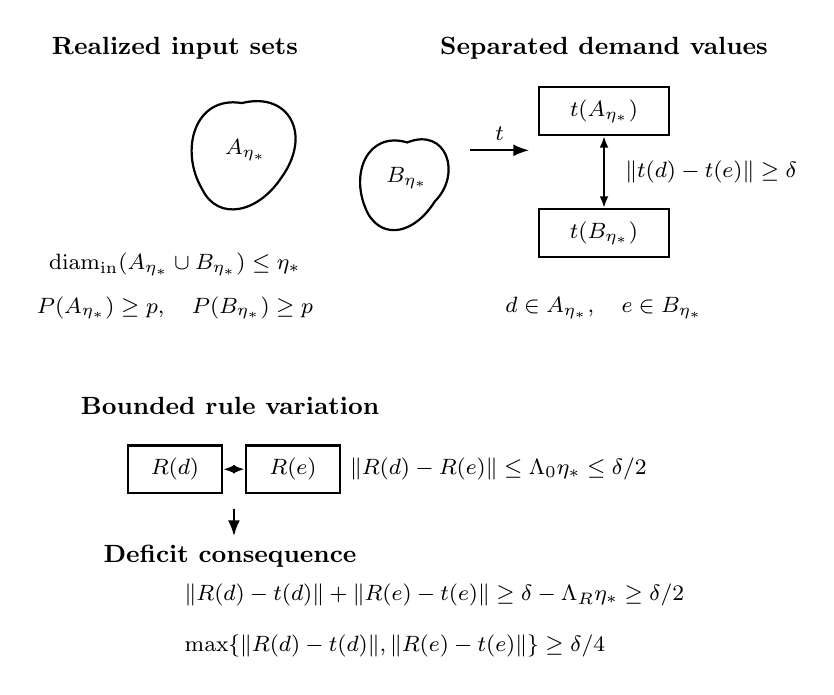
\begin{tikzpicture}[
  x=1cm, y=1cm,
  font=\footnotesize,
  stage/.style={font=\small\bfseries},
  set/.style={draw, thick},
  map/.style={-{Latex[length=2mm]}, thick},
  bound/.style={{Latex[length=1.5mm]}-{Latex[length=1.5mm]}, thick}
]
% Realized input sets and their separated demand values.
\node[stage] at (0,3.7) {Realized input sets};
\draw[set] (0.35,1.9) .. controls (0.05,2.4) and (0.25,3.1) .. (0.85,3.0)
  .. controls (1.45,3.15) and (1.75,2.6) .. (1.35,2.05)
  .. controls (1.05,1.6) and (0.55,1.5) .. cycle;
\node at (0.9,2.4) {$A_{\eta_*}$};
\draw[set] (2.45,1.6) .. controls (2.2,2.1) and (2.45,2.65) .. (2.95,2.5)
  .. controls (3.45,2.7) and (3.65,2.1) .. (3.3,1.75)
  .. controls (3.05,1.35) and (2.65,1.25) .. cycle;
\node at (2.95,2.05) {$B_{\eta_*}$};
\node[align=left] at (0,0.95)
  {$\mathrm{diam}_{\mathrm{in}}(A_{\eta_*}\cup B_{\eta_*})\leq\eta_*$};
\node[align=left] at (0,0.4) {$P(A_{\eta_*})\geq p,\quad P(B_{\eta_*})\geq p$};

\node[stage] at (5.45,3.7) {Separated demand values};
\node[set, minimum width=4.7em, minimum height=4ex] (ta) at (5.45,2.9)
  {$t(A_{\eta_*})$};
\node[set, minimum width=4.7em, minimum height=4ex] (tb) at (5.45,1.35)
  {$t(B_{\eta_*})$};
\draw[bound] (ta) -- node[right, xshift=4pt]
  {$\|t(d)-t(e)\|\geq\delta$} (tb);
\node at (5.45,0.4) {$d\in A_{\eta_*},\quad e\in B_{\eta_*}$};

\draw[map] (3.75,2.4) -- node[above] {$t$} (4.5,2.4);

% The same pair under the bounded-description rule, followed by the deficit.
\node[stage] at (0.7,-0.85) {Bounded rule variation};
\node[set, minimum width=3.4em, minimum height=4ex] (ra) at (0,-1.65)
  {$R(d)$};
\node[set, minimum width=3.4em, minimum height=4ex] (rb) at (1.5,-1.65)
  {$R(e)$};
\draw[bound] (ra) -- (rb);
\node[anchor=west] at (2.1,-1.65)
  {$\|R(d)-R(e)\|\leq\Lambda_0\eta_*\leq\delta/2$};
\node[stage] at (0.7,-2.75) {Deficit consequence};
\draw[map] (0.75,-2.15) -- (0.75,-2.5);
\node[anchor=west] at (0,-3.25)
  {$\|R(d)-t(d)\|+\|R(e)-t(e)\|\geq\delta-\Lambda_R\eta_*\geq\delta/2$};
\node[anchor=west] at (0,-3.9)
  {$\displaystyle\max\{\|R(d)-t(d)\|,\|R(e)-t(e)\|\}\geq\delta/4$};
\end{tikzpicture}
\caption{Schematic of P4 and the risk-gap argument at the realized scale $\eta_*$ (not empirical certification). Sets need not be intervals or connected. Realization gives probability at least $p$ to a deficit of $\delta/4$ or more, so $\mathrm{risk}(R)\geq p\delta^2/16$; the gap floor $\kappa=p\delta^2/16-\rho$ is positive only when $\rho<p\delta^2/16$.}
\label{fig:p4-geometry}
\end{figure}

The one-scale quantifier is essential. Requiring instead $P(A_\eta),P(B_\eta)\geq p>0$ at \emph{every} $\eta>0$ would make the usual non-atomic Euclidean Borel model vacuous. For independent $D,E\sim P$, disjointness and the diameter bound imply $P\times P(0<d_{\mathrm{in}}(D,E)\leq\eta)\geq p^2$ for every $\eta$, whereas these nested events decrease to the empty set as $\eta\downarrow0$ and their probabilities tend to zero. The present formulation removes that contradictory all-scales requirement.

The repaired conditions are consistent. For example, take instances in $[-1,1]$ with uniform $P$, scalar demand $t(d)=0$ for $d\leq0$ and $t(d)=\delta$ for $d>0$, and $h=\min\{\eta,1\}$. The sets $A_\eta=(-h/2,0)$ and $B_\eta=(0,h/2)$ have union diameter at most $\eta$, demand separation $\delta$, and probability $h/4$ each. Choosing a sufficiently small $\eta_*$ satisfies \eqref{eq:realization} for any prescribed finite $\Lambda_0$, with $p=\eta_*/4$. This mathematical example does not establish P4 for a real inverse problem or establish that the resulting $\kappa$ below is positive.

\begin{uprop}[Barrier to Gap]
Suppose P4a \eqref{eq:barrier} holds with separation $\delta$, BD \eqref{eq:rate} holds uniformly on $\mathcal{C}$ with rate $\Lambda_0$, and scale-restricted P4b \eqref{eq:realization} holds at $\eta_*$ and level $p$. Then every $R\in\mathcal{C}$ satisfies
\begin{equation}
\mathrm{risk}(R)\geq\frac{p\delta^2}{16}, \qquad\text{and hence}\qquad g(R)\geq\frac{p\delta^2}{16}-\rho=\kappa,
\label{eq:floor}%
\end{equation}%
where $\rho$ is any upper bound on the fixed benchmark risk $\mathrm{risk}^*$. If $\rho<p\delta^2/16$, then $\kappa>0$, the risk gap is at least $\kappa$ uniformly on $\mathcal{C}$, and Lemma 3 excludes uniform $\epsilon$-accuracy for every $R\in\mathcal{C}$ and every $0<\epsilon<\kappa$.
\label{prop:barrier}%
\end{uprop}

\argument Fix $R\in\mathcal{C}$ with rate $\Lambda_R\leq\Lambda_0$, and use the realized scale $\eta_*$; no limiting scale selection is needed. Write $A=A_{\eta_*}$ and $B=B_{\eta_*}$. For $d\in A$ and $e\in B$, the triangle inequality gives
\begin{equation}
\|R(d)-t(d)\|+\|R(e)-t(e)\|\geq\|t(d)-t(e)\|-\|R(d)-R(e)\|\geq\delta-\Lambda_R\eta_*\geq\frac{\delta}{2},
\label{eq:deficit}%
\end{equation}%
where the last step uses $\Lambda_R\eta_*\leq\Lambda_0\eta_*\leq\delta/2$, including the case $\Lambda_0=0$ without division. Hence at least one member of every pair has deficit at least $\delta/4$. The set $S$ of instances with deficit at least $\delta/4$ therefore contains all of $A$ or all of $B$: otherwise choosing $d\in A\setminus S$ and $e\in B\setminus S$ would contradict \eqref{eq:deficit}. By \eqref{eq:realization}, $P(S)\geq p$, so $\mathrm{risk}(R)\geq p(\delta/4)^2$. The gap bound follows from \eqref{eq:gap} and $\mathrm{risk}^*\leq\rho$, and the tolerance assertion follows from Lemma 3.\qedbox

The same $\kappa$ applies to every member of $\mathcal{C}$ and termwise to any sequence that remains in $\mathcal{C}$. This does not contradict universal-approximation theorems, which concern different target classes, topologies, losses, and hypotheses. Nor does a finite budget of frozen metaparameters create a third provenance mode: such a component remains Mode B and is included only if it belongs to the specified BD class. Finite-resolution experiments cannot certify the every-scale barrier P4a, and realization probabilities and the benchmark must be estimated separately before a numerical $\kappa$ can be claimed.

\subsection{Classification and Collision: Neural Networks}

Inference by a neural network feeds the current input into a set of weights in a forward computation; the weights do not change at inference time, and their values come from the statistics of a training corpus or from manual setting.

\begin{proposition}
The context rule of a neural network whose content-carrying values are corpus-statistical or manually set and fixed at inference belongs to Mode~B. Separately, if $d,e$ are a mask-collision pair with $d|_{\ev}=e|_{\ev}$ and different candidate context, and the rule exhibits \emph{collision output variation}, namely $\exists i\in I$ such that $R_i(d)\neq R_i(e)$, then it cannot have the A1 evidence-only behavior \eqref{eq:modeA} on that pair.
\label{prop:modeB}%
\end{proposition}

\argument The network's rule satisfies \eqref{eq:modeB}, with $W$ the weights and $F_i$ forward propagation; corpus-statistical or manually set frozen content determines Mode~B by provenance. For the collision assertion, \eqref{eq:modeA} would force $R_i(d)=R_i(e)$ at every position, contradicting output variation. Nonzero weights alone do not imply this variation, and small weights do not imply degeneracy: output variation must be checked for the specified pair. The argument excludes an A1 evidence-only realization, not A2 candidate-adaptive analytic behavior \eqref{eq:modeA2}. A network computing only a fixed analytic function of evidence and candidate context can still be Mode~A by the analytic-invariant clause; a frozen corpus-trained network that happens to implement such a function remains Mode~B by provenance.\qedbox

\begin{theorem}
Use the fixed test distribution, measurable demand $t$ and rules, integrable squared loss, and fixed benchmark $\mathrm{risk}^*$ of Lemma~3. Let $\mathcal{C}$ be a specified class of offline-frozen neural-network context rules whose content-carrying values are corpus-statistical or manual, satisfying uniform BD, P4a, and scale-restricted P4b, with $\rho\ge\mathrm{risk}^*$ a fixed benchmark bound and $\kappa=p\delta^2/16-\rho>0$. Then no $R\in\mathcal{C}$ is uniformly $\epsilon$-accurate for any $0<\epsilon<\kappa$. Thus a solo network in this class cannot independently meet this $\epsilon$-complete open-inversion requirement. This is a class-level bound: it neither establishes nor refutes Hypothesis~$\mathcal{H}_{\mathrm{NN}}$ outside $\mathcal{C}$, and it does not cover arbitrary tasks, networks, or tolerances.
\label{thm:main}%
\end{theorem}

\argument Barrier-to-Gap gives $g(R)\geq\kappa$ for every $R\in\mathcal{C}$. For any $0<\epsilon<\kappa$, $g(R)>\epsilon$, so Lemma~3 contradicts uniform $\epsilon$-accuracy. The bound uses P4a for the separation, BD for the uniform rate, P4b for positive mass at the realized scale, and the benchmark bound for $\kappa>0$. Collision output variation is not used in the bound; it is a separate definitional check that excludes A1, not A2, on a specified pair. In particular, P1--P3 alone, nonzero weights, or a bound at one larger tolerance would not suffice.\qedbox

\subsection{A Nonvacuous Instance}
\label{sec:instance}%

The consistency example before Proposition~4 shows that P4b need not contradict a non-atomic $P$, but it does not supply a class $\mathcal{C}$ or a positive floor. A complete formal witness is small. Let $I=\{1,2\}$, let position $1$ be the evidence part and position $2$ the mask hole, and put
\begin{equation}
t(d)=\bigl(\delta\,\mathbf{1}\{d_1>0\},\,0\bigr),
\qquad
\mathcal{C}=\bigl\{R_a(d)=(a\,d_1,\,a\,d_2): \tfrac12\le a\le 1\bigr\},
\label{eq:witness}%
\end{equation}
with $\delta>0$, $P$ uniform on $[-1,1]^2$, and $d_{\mathrm{in}}$ the sup norm. Each $R_a$ is a one-layer linear network whose weight is set manually and frozen at inference, hence Mode~B by provenance; its rate is $\Lambda_R=a\le 1$, so $\Lambda_0=1$. On the collision pair $d=(0,0)$ and $e=(0,1)$, the evidence $d_1=0$ is the same, while $R_a(e)-R_a(d)=(0,a)\neq(0,0)$, so collision output variation holds. The class is deliberately linear and cannot represent the step in $t$; this is the source of its positive risk.

For every $\eta>0$, put $h=\min\{\eta,1\}$ and set
\[
A_\eta=(-h/2,0)\times[-h/4,h/4],
\qquad
B_\eta=(0,h/2)\times[-h/4,h/4].
\]
Their union has sup-norm diameter at most $h\le\eta$, and $\|t(d)-t(e)\|\ge\delta$ for $d\in A_\eta$, $e\in B_\eta$, so P4a holds at every scale. Uniformity gives $P(A_\eta)=P(B_\eta)=h^2/16$. Choose $\eta_*\le\min\{1,\delta/2\}$ and $p=\eta_*^2/16$; then P4b holds with $\Lambda_0\eta_*\le\delta/2$. The benchmark class $\mathcal{A}$ may contain $t$ itself, which is measurable and evidence-instantiated because it depends only on $d_1$; then $\mathrm{risk}^*=0$, and the floor is $\kappa=p\delta^2/16>0$. The theorem therefore excludes every rule in $\mathcal{C}$ for every $0<\epsilon<\kappa$.

This witness is deliberately abstract: it proves that the hypotheses are jointly satisfiable and that the theorem is not vacuous, not that a real inverse problem has this demand. In particular, $t$ is a step function, and no empirical procedure can certify its every-scale barrier from finite samples. A real application must supply its own mask model, demand, class, and benchmark, and must justify why the step-like behavior is a defensible model of the task rather than an artifact of the construction.

\emph{An edge-aware denoising reading.}
The algebra has a practical reading that motivates the hypotheses without verifying them. Consider a one-dimensional image row with an intensity edge and a mask hole that straddles the edge. The observed pixels on the two sides determine which side is the boundary and which is the interior; a smoothing rule should therefore use a different strength on each side. A single global coefficient must either over-smooth the edge or under-smooth the interior, which is the stationarity-ratio obstruction of Lemma~1. A position-wise table can encode two strengths, but only for configurations that place the boundary at the same position; if the evidence flips which side is boundary, the table's fixed assignment becomes the wrong assignment, which is the cross-configuration failure of \eqref{eq:tablecondition}. An edge detector that reads the observed sides and sets the strength analytically is Mode~A1 or A2; a denoiser whose strengths were fitted to a corpus of edges remains Mode~B even when it is fast and accurate in distribution.

This reading also predicts where the risk should concentrate: near edges whose location is not determined by the training distribution, a frozen rule should show an oracle excess that grows when the edge moves, and a per-position table should degrade when the evidence reverses the two sides. Those predictions are testable in a controlled inpainting or depth-completion study, but the present paper does not run such a study and does not use the reading as evidence for P4a or for a numerical $\kappa$. The two-position witness above is a minimal algebraic abstraction of the mechanism, not a calibrated image model.

On the four-position toy carrier of the machine-verification artifact, two illustrative demands give total-loss comparisons between frozen coefficients and constructive evidence-instantiated rules. These toy computations illustrate the provenance distinction; they do not verify BD, P4, the general neural class, or the quantitative floor of Theorem~5.

Beyond the algebra, the exclusion does not depend on the dimension of the parameter object: a position-wise or layer-wise table is Mode~B of higher dimension, and \eqref{eq:tablecondition} excludes a frozen family across two configurations only when its zero-safe compatibility conditions fail. On the nondegenerate locus, one position whose defined stationarity ratio changes is sufficient. Approximate inference---loopy belief propagation, structured variational inference, learned proposals---changes cost and accuracy, not provenance. Composite systems containing Mode~A are not ruled out, but their completeness is not proved by this result and must be established separately.

\subsection{Verification Scope}
\label{sec:verification}

The algebraic core and a toy-carrier closure are machine-verified in Lean~4 with Mathlib, with no \texttt{sorry}, no project-specific axiom, and only Lean's standard axioms \citep{demoura2021,mathlib2020}. The artifact proves the proportionality identities behind Lemma~1, the unconstrained Paradigm~I minimizer, a support-restricted single-rule form of Lemma~3, and a scalar toy closure; it does not prove the general neural Theorem~\ref{thm:main}, BD, P4a/P4b, Barrier-to-Gap, or any real-world modeling premise. It also defines task-level P2 and support-level P3 predicates and checks that neither implies P1 or mask openness, respectively. Appendix~\ref{app:verification} gives the declaration mapping and separates verified algebra from the analytic residue.

\section{Discussion}
\label{ch:discussion}%

The Mode~B phenomenon has an everyday form: deep networks can fit random labels with near-zero training error, so frozen weights can store a corpus's numerical table \citep{zhang2021}. That observation motivates the provenance question but does not answer it. A synthetic reconstruction probe is not evidence for the theorem either: reconstruction RMSE is not the squared rule-value gap $g(R)$, a finite sample cannot certify the every-scale barrier P4a, and a single constructed task cannot estimate the benchmark risk $\mathrm{risk}^*$ over the full evidence-instantiated class. Accordingly, the paper makes no empirical claim of that kind and does not use a synthetic probe as confirmation of Theorem~5.

\subsection{Evaluation Protocol}
\label{sec:protocol}%

For a concrete task, the result is used as a protocol rather than as a blanket verdict.

\begin{enumerate}
\item \emph{Check the base class.} Establish P1 (the observation admits multiple structures), P2 (the required strength is heterogeneous and evidence-addressed), and P3 (test inputs are not confined to the training distribution). If any fails, the theorem does not apply.
\item \emph{Fix the evaluation objects before seeing results.} Specify the test distribution $P$, the metric $d_{\mathrm{in}}$, the benchmark class $\mathcal{A}$ of evidence-instantiated rules, and the candidate class $\mathcal{C}$ of offline-frozen rules. The benchmark must be fixed independently of $\mathcal{C}$ and must not contain the candidate rule being evaluated; otherwise $\mathrm{risk}^*$ can be made equal to $\mathrm{risk}(R)$ and the gap trivial.
\item \emph{Estimate the three quantitative inputs.} Bound the uniform rate $\Lambda_0$ from the architecture and weight ranges, estimate the realized mass $p$ at a candidate scale, and bound $\mathrm{risk}^*$ from the benchmark. Choose $\rho\ge\mathrm{risk}^*$ and compute $\kappa=p\delta^2/16-\rho$.
\item \emph{Read the conclusion at the stated tolerance.} If $\kappa>0$, no $R\in\mathcal{C}$ is uniformly $\epsilon$-accurate for any $0<\epsilon<\kappa$. If $\kappa\le0$, the theorem is silent; this is not evidence that a frozen rule is complete.
\item \emph{Report what is not identified.} P4a is a modeling assumption about all scales, not a finite-sample estimate; $t$ is generally unobserved at deployment; and the bound is relative to the chosen $P$, $\mathcal{A}$, and metric. Report sensitivity to those choices rather than a single number.
\end{enumerate}

\begin{table}[!ht]
\caption{Protocol inputs: what is fixed, what is estimated, and what remains a modeling assumption. The table makes the division of labor explicit; it is not a claim that every row is identifiable from one data set.}
\label{tab:protocol}
\centering
\small
\begin{tabular}{@{}>{\raggedright\arraybackslash}p{0.20\textwidth}>{\raggedright\arraybackslash}p{0.30\textwidth}>{\raggedright\arraybackslash}p{0.42\textwidth}@{}}
\hline
\textbf{Input} & \textbf{How it is fixed} & \textbf{Evidential status}\\
\hline
$P$ & Test distribution and support, before seeing results & Estimated from a test sample; unsupported regions are outside the claim.\\
$\mathcal{A}$ & Evidence-instantiated benchmark class, independent of $\mathcal{C}$ & Defined by the protocol; must not contain the candidate rule.\\
$\mathcal{C}$ & Specified offline-frozen class, including weight range & Membership is checkable; uniform BD is a separate assumption.\\
$d_{\mathrm{in}}$ & Domain metric on structure fields & Chosen, not estimated; report sensitivity to the choice.\\
$\delta$ & Demand separation from the task model & A modeling assumption; finite samples cannot certify it at every scale.\\
$p$ & Realized mass at one admissible scale $\eta_*$ & Estimable at a fixed scale, with sampling uncertainty.\\
$\mathrm{risk}^*$ & Benchmark risk of the best evidence-instantiated rule & Estimable from the benchmark sample; not a property of $\mathcal{C}$.\\
$\kappa$ & Computed as $p\delta^2/16-\rho$ & A derived quantity; report its sensitivity, not a single certificate.\\
\hline
\end{tabular}
\end{table}

A masked image-inpainting or depth-completion study illustrates the mapping. The mask fixes the evidence part and leaves context positions free (P1); the required smoothing strength varies at depth edges and occlusion boundaries (P2); test images can leave the training distribution (P3). A frozen CNN or position-wise table is a candidate class $\mathcal{C}$; analytic, calibration, or SURE-type rules form an evidence-instantiated benchmark $\mathcal{A}$ \citep{stein1981,romano2017}. In a controlled data set with ground-truth structure one can estimate $p$ and $\mathrm{risk}^*$ and check whether $\kappa>0$; at deployment $t$ is not observed, so the resulting $\kappa$ is a modeling quantity, not a deployable certificate. Reconstruction error can be reported alongside, but it is not $g(R)$ and does not replace the protocol.

\subsection{Existence, Cost and Design Implications}
\label{sec:cost}%

Whether Mode A exists determines the practical reading of the conclusion: the analytic-invariant path takes its values directly from calibration and geometry, and the per-instance optimization path solves the rule values separately for each input \citep{sun2020}. Analytic evaluation is often cheaper than iterative per-instance optimization, but the actual cost depends on scale, accuracy, hardware, and stopping conditions; no universal cost factor is claimed. This tradeoff motivates composite systems: Mode B in cost-sensitive and in-distribution stages, Mode A in the critical stage of rule generation. Three questions then follow for design: where the rule's values come from; whether they are frozen at inference time; and who on the open set instantiates the rule. A positive completeness claim additionally requires A0 and a correctness proof for the proposed Mode A mechanism.

Three limitations delimit the result. First, P4a, uniform BD, scale-restricted P4b, and $\rho<p\delta^2/16$ are load-bearing hypotheses. Tasks with Lipschitz or exactly corpus-identifiable demand, discontinuous frozen rules outside the BD class, or inadequate realization or benchmark bounds are outside the quantitative exclusion; the theorem is then silent, not proof that a frozen rule is complete. Second, the positive claims need Assumption A0, which tasks whose demand depends on unobserved structure fail. Third, the negative result concerns solo use within the specified class: composites containing Mode A are not ruled out, but neither their completeness nor the interaction of their components is proved here.

\section{Conclusion}
\label{ch:conclusion}%

For a fixed test distribution and squared rule-value loss, a fixed evidence-instantiated benchmark, and a specified offline-frozen class satisfying uniform BD, P4a, and scale-restricted P4b, a positive $\kappa=p\delta^2/16-\rho$ excludes uniform $\epsilon$-accuracy throughout that class for every $0<\epsilon<\kappa$. This is a conditional result about independent task solving, not a denial of in-distribution usefulness, not logic completeness, and not a consequence of P1--P3 alone. If the comparison class exhausts the offline-frozen Mode B alternatives that satisfy these hypotheses, an admitted rule meeting the bound must be Mode~A (A1 or A2); Mode~A membership alone is not sufficient for correctness.

Lemma 1 excludes a shared scalar when cross-position stationarity ratios differ and gives the zero-safe two-configuration compatibility condition for a frozen position-wise family; heterogeneity at one configuration alone does not exclude such a family. Lemma 2 separates objective form from provenance, and Lemma 3 supplies the conditional risk argument. Proposition 4 classifies corpus- or manually parameterized frozen networks as Mode B and uses output variation, rather than nonzero weights, for the separate collision statement. Theorem 5 combines these pieces only with the stated class, benchmark, and tolerance hypotheses. The Lean artifact verifies algebraic components and a toy closure, not the general analytic or empirical premises.

The same classification can be applied to Markov random fields, conditional random fields, mixtures, dictionary learning, and kernel methods, but the quantitative exclusion follows only when their rules belong to a class satisfying the theorem's hypotheses. Online updating alone does not imply Mode A: evidence plus analytic or calibration invariants is Mode A, while corpus-statistical or manual frozen content remains Mode B, including a corpus-fitted generator of online updates. Tasks outside P4 or BD are not thereby shown to admit complete frozen solvers. Composite systems containing Mode A remain possible and require separate correctness arguments. Negation is therefore not disparagement: it is a scoped boundary claim, with constructive design and standardized empirical evaluation left as future work.

Three lessons follow. First, provenance is not capacity: the question is not how many parameters a component has, but whether the values that carry its context can be regenerated from the evidence at inference time. Second, benchmark accuracy is not open-set completeness: a frozen rule can be accurate in distribution and still fail the independent-task requirement once P2 and P3 are active. Third, frozen sufficiency is an identifiability question: it requires a demand model, a comparison class, a uniform rate, a realized scale, and a benchmark, and the absence of any one of these leaves the theorem silent rather than proving completeness. These lessons turn the negative result into a design checklist: establish provenance, state the demand model, and test the bound only where its inputs are identifiable.

\acks{The authors would like to sincerely thank all participants who provided valuable suggestions for optimizing the work presented in this paper. This research was financially supported by the National Natural Science Foundation of China (Grant nos. 52306144, 72404254, and 72604262), the University-Enterprise Cooperative Research Fund with DALIAN WINDTUNER TECHNOLOGY CO.,LTD. (Grant No. 20231061030006), the Shenzhen Science and Technology Program (Grant nos. KCXFZ20230731093902005, JCYJ20241202124703004, CJGJZD20250902091259006, and KJZD20240903103806009), the Guangdong Basic and Applied Basic Research Foundation (Grant 2026A1515010187), and the Guangdong Provincial Key Laboratory of Low-Altitude Intelligent Perception and Navigation Safety (No. 2026B1201010001).

The verified artifact described in Appendix~\ref{app:verification} was developed with the Lean~4 proof assistant and its mathematical library Mathlib, and is distributed in the \texttt{lean-proof} directory of the repository with the \texttt{lean-toolchain} file that pins the toolchain version.

Competing interests: the authors declare no competing interests.}

\appendix
\section{Complete Proofs}
\label{app:proofs}

The main text gives proof sketches to keep the argument visible. This appendix records the complete derivations, including the zero-coefficient cases and the measure-theoretic step.

\subsection{Proof of Lemma~\ref{lem:scalar}}
For the quadratic objective \eqref{eq:paradigmE}, differentiating with respect to $z_i$ gives
\[
2(z_i-x_i)+2\lambda\sum_{j\in I}2(z_i-z_j)=0,
\]
which is \eqref{eq:foc}. If one scalar $\lambda$ satisfies \eqref{eq:foc} at positions $i$ and $j$, then
\[
x_i-z_i=2\lambda c_i(z),\qquad x_j-z_j=2\lambda c_j(z).
\]
Eliminating $\lambda$ gives \eqref{eq:proportion}. When the stationarity ratios $q_i(z)=-f_i'(z_i)/c_i^\varphi(z)$ and $q_j(z)$ are defined and differ, no common $\lambda$ can satisfy both equations. The condition is necessary for stationarity; no convexity or global-minimizer claim is used.

For the general separable objective, the derivative of the ordered sum is
\[
\frac{\partial}{\partial z_i}\sum_{a,b}\varphi(z_a-z_b)
=2\sum_{j}\varphi'(z_i-z_j)=c_i^\varphi(z),
\]
where the factor two uses that $\varphi$ is even, hence $\varphi'$ is odd. Thus \eqref{eq:focgeneral} is the stationarity condition.

For a frozen family, set $a=f_i'(z_i)$, $a'=f_i'(z'_i)$, $b=c_i^\varphi(z)$, and $b'=c_i^\varphi(z')$. A common $W_i$ must satisfy $a+W_i b=0$ and $a'+W_i b'=0$.
If $b,b'\neq0$, eliminating $W_i$ gives $ab'=a'b$. If $b=0$, the first equation gives $a=0$; when $b'\neq0$, the second determines $W_i=-a'/b'$. If $b'=0$, the second gives $a'=0$. If $b=b'=0$, both $a=a'=0$ and any $W_i$ works. These are exactly the three lines of \eqref{eq:tablecondition}. Conversely, in each case choose $W_i=-a/b$ if $b\neq0$, otherwise $W_i=-a'/b'$ if $b'\neq0$, and arbitrary when both vanish; the implications make the chosen value satisfy both equations. This proves the equivalence. On the nondegenerate locus, $W_i=q_i(z)=q_i(z')$.

\subsection{Proof of Lemma~\ref{lem:objective}}
The quadratic Paradigm~E objective is a sum of a positive definite data term and a positive semidefinite consistency term; for $\lambda>0$ it is strictly convex and coercive on $\mathbb{R}^{I}$, hence has a unique minimizer. The minimizer can be biased because the consistency term is not the demand itself.

At one configuration, if $c_i^\varphi(z)\neq0$, choosing $W_i=-f_i'(z_i)/c_i^\varphi(z)$ satisfies \eqref{eq:focgeneral} at every position; if $c_i^\varphi(z)=0$, stationarity requires $f_i'(z_i)=0$. Hence a frozen table can fit a single configuration by construction, and heterogeneity at that configuration alone does not exclude it. Across two configurations, the existence of one common table is exactly the equivalence in \eqref{eq:tablecondition}; failure of any line excludes the table.

For Paradigm~I, $\mathcal{I}(x,p)=\sum_i(x_i-p_i)^2\ge0$, with equality iff $p_i=x_i$ for every $i$. This proves the unconstrained case. If $p=G_\theta(x)$ is constrained to a range or latent parameterization, the equality conditions need not be attainable; existence and uniqueness then require range, injectivity, or convexity hypotheses. Since both paradigms can be implemented by analytic weights or by corpus-fitted tables, neither objective form determines provenance.

\subsection{Proof of Lemma~\ref{lem:risk}}
Uniform $\epsilon$-accuracy gives $\ell(R,d_0)\le\epsilon$ at the realized input $d_0$. Upper-tail realization gives $\mathrm{risk}(R)\le\ell(R,d_0)$, hence $\mathrm{risk}(R)\le\epsilon$. On the other hand, $\mathrm{risk}^*\ge0$ and \eqref{eq:gap} give
\[
\mathrm{risk}(R)=g(R)+\mathrm{risk}^*>g(R)>\epsilon,
\]
a contradiction. For a class, the same argument applies to every $R\in\mathcal{C}$ with $g(R)\ge\kappa$ and every $0<\epsilon<\kappa$. If one adds the separate assumption that $\mathcal{C}$ exhausts the admissible offline-frozen alternatives, an admitted rule meeting the accuracy claim cannot lie in $\mathcal{C}$; it must be Mode~A (A1 or A2). That is a design-level corollary of the extra partition assumption, not a consequence of Theorem~\ref{thm:main}, and it does not say that every evidence-instantiated rule is correct.

Upper-tail realization holds for an integrable loss on a finite support and for a non-atomic support under the stated measurability and integrability assumptions: the mean is not larger than the essential supremum, and the set on which the loss is at least its mean has positive probability. The benchmark must be fixed independently of the candidate; otherwise the gap can be made trivial.

\subsection{Proof of Barrier-to-Gap}
Fix $R\in\mathcal{C}$ and use the realized scale $\eta_*$ rather than a limit. For $d\in A_{\eta_*}$ and $e\in B_{\eta_*}$,
\[
\|R(d)-t(d)\|+\|R(e)-t(e)\|
\ge\|t(d)-t(e)\|-\|R(d)-R(e)\|
\ge\delta-\Lambda_R\eta_*
\ge\frac{\delta}{2},
\]
where the last inequality uses $\Lambda_R\le\Lambda_0$ and $\Lambda_0\eta_*\le\delta/2$; if $\Lambda_0=0$, the inequality is immediate. Hence at least one of $d,e$ has deficit at least $\delta/4$. Let $S$ be the set of inputs with deficit at least $\delta/4$. If neither $A_{\eta_*}$ nor $B_{\eta_*}$ were contained in $S$, choosing $d\in A_{\eta_*}\setminus S$ and $e\in B_{\eta_*}\setminus S$ would make both deficits smaller than $\delta/4$ and contradict the displayed inequality. Thus $S$ contains one of the two sets, so $P(S)\ge p$ by \eqref{eq:realization}. Therefore
\[
\mathrm{risk}(R)=\mathbb{E}_P\|R-t\|^2
\ge(\delta/4)^2P(S)
\ge\frac{p\delta^2}{16}.
\]
Since $\mathrm{risk}^*\le\rho$, $g(R)=\mathrm{risk}(R)-\mathrm{risk}^*\ge p\delta^2/16-\rho=\kappa$. Lemma~\ref{lem:risk} then excludes uniform $\epsilon$-accuracy for every $0<\epsilon<\kappa$.

The discarded all-scales formulation required $P(A_\eta),P(B_\eta)\ge p$ at every $\eta>0$. For independent $D,E\sim P$, the event $D\in A_\eta,E\in B_\eta$ has probability at least $p^2$ and implies $0<d_{\mathrm{in}}(D,E)\le\eta$. These nested events decrease to the empty set as $\eta\downarrow0$, so their probabilities tend to zero, contradicting the uniform lower bound $p^2$. The scale-restricted condition retains the quantitative content without this inconsistency.

\subsection{Proof of the Collision Proposition and Theorem~\ref{thm:main}}
A corpus- or manually parameterized network has rule values fixed at inference time and determined by training statistics or manual setting, so it satisfies the Mode~B clause of Definition~3. If it also satisfied the evidence-only behavior \eqref{eq:modeA} on a collision pair $d,e$ with $d|_{\ev}=e|_{\ev}$, then $R_i(d)=R_i(e)$ for every $i$, contradicting the assumed output variation at some $i$. The argument uses output variation, not nonzero weights: a network with nonzero weights can be constant on the pair, and a network with small weights can vary there.

For Theorem~\ref{thm:main}, Each $R\in\mathcal{C}$ is Mode~B by its corpus or manual provenance, and the collision statement is separate. Barrier-to-Gap gives $g(R)\ge\kappa$ uniformly. Lemma~\ref{lem:risk} then contradicts uniform $\epsilon$-accuracy for $0<\epsilon<\kappa$. The accuracy bound uses P4a for the separation, BD for the uniform rate, P4b for positive mass at the realized scale, and the benchmark bound for $\kappa>0$. Collision output variation is not used in that bound; it only supports the separate, definitional statement about A1 behavior. If $\kappa\le0$, the argument is silent.

\section{Lean Artifact and Declaration Map}
\label{app:verification}

The artifact is in the \texttt{lean-proof} directory of the repository \url{https://github.com/aki-xavier/frozen-axis}. It is built with \texttt{lake build} on Lean~4.35.0 and Mathlib at the matching release; the declarations below are checked without \texttt{sorry} or project-specific axioms. The artifact is a formal companion, not a proof of the modeling premises.

\begin{table}[t]
\caption{Lean~4 verification coverage. Tiers A and B identify formalized components; Tier C is the uncovered analytic and modeling residue. The toy declarations \texttt{theorem5} and \texttt{finale} do not verify the general Theorem~\ref{thm:main}, BD, P4, or real-task premises.}
\label{tab:verification-tiers}
\centering
\small
\begin{tabular}{@{}>{\raggedright\arraybackslash}p{0.24\textwidth}>{\raggedright\arraybackslash}p{0.70\textwidth}@{}}
\hline
\textbf{Tier} & \textbf{Covered content or residue}\\
\hline
A: carrier-independent algebra & Lemma~1's proportionality identities and general first-order condition; mode-composition steps used in the toy closure.\\
\hline
B: single-rule algebra and measure lemmas & Ill-posedness and collision constructions; the unconstrained Paradigm~I minimizer; the fixed-benchmark, test-support single-rule risk lemma; \texttt{tail\_realization}. Not the class-level Lemma~3.\\
\hline
C: not machine-verified & Continuous-side Euler--Lagrange arguments; general network output variation; the zero-safe table equivalence in general form; BD, P4a/P4b, and Barrier-to-Gap.\\
\hline
\end{tabular}
\end{table}

The algebraic skeleton and a toy-carrier closure are machine-verified, with no \texttt{sorry}, no project-specific axiom, and only Lean's standard axioms. The declarations \texttt{theorem5} and \texttt{finale} concern the scalar toy rule $\texttt{neuralRule}\ W\ d=W(d_0-d_1)$ with $W\neq0$; \texttt{finale} additionally assumes a support-restricted tail, a positive gap, and benchmark nonnegativity. The artifact does not prove general neural-network output variation, BD, P4a/P4b, Barrier-to-Gap, or any real-world modeling premise.

The artifact separately defines task-level predicates. \texttt{Task} carries an observation, a current depth, a demand profile, a boundary predicate, and training and test supports. \texttt{P2} requires the demand and boundary to be evidence-addressed and to differ between a boundary and an interior position at the current depth; \texttt{P3} requires a test input outside the training support. The finite witnesses \texttt{flipTask} and \texttt{inpaintTask} satisfy P1 and these task-level predicates. Their Lean tasks fix a finite position set but define no probability measure or metric on test instances; they therefore neither establish nor refute the every-scale P4a condition, and they do not instantiate Theorem~\ref{thm:main}. They show that the formal base class is nonempty, not that a real deployment satisfies P2 or P3.

The toy predicates \texttt{MaskOpen},\allowbreak\ \texttt{Hetero}\allowbreak\texttt{Kappa},\allowbreak\ \texttt{IsEvidence}\allowbreak\texttt{OnlyToy},\allowbreak\ and \texttt{IsFrozen}\allowbreak\texttt{ScalarToy} are deliberately narrower than the paper's P3, P2, and provenance classes. The first is a mask-openness bridge, the second is a concrete coefficient-heterogeneity condition, and the last two are behavioral projections used by the scalar closure. The paper's claims about the general class remain analytic, and the Lean development is cited only for the algebra and the finite bases it actually checks.

\section{A Worked Risk Calculation}
\label{app:calculation}

The witness of Section~\ref{sec:instance} can be evaluated explicitly, which shows the size of the floor and its sensitivity to the benchmark. Take $\delta=1$, $\eta_*=1/4$, and $h=\eta_*$. Then
\[
p=P(A_{\eta_*})=P(B_{\eta_*})=\frac{h^2}{16}=\frac{1}{256},
\qquad
\kappa=\frac{p\delta^2}{16}=\frac{1}{4096}.
\]
The class $\mathcal{C}=\{R_a(d)=(a d_1,a d_2):1/2\le a\le1\}$ has
\[
\mathrm{risk}(R_a)=\frac{2a^2}{3}-\frac{a\delta}{2}+\frac{\delta^2}{2}.
\]
At position~1 the squared error is $(a d_1-\delta\mathbf{1}\{d_1>0\})^2$, whose mean is $a^2/3-a\delta/2+\delta^2/2$; position~2 contributes $a^2/3$. With $\delta=1$ the best member is $a=1/2$, with risk $5/12\approx0.417$. If the benchmark class contains $t$, then $\mathrm{risk}^*=0$ and the actual gap is $5/12$, far above the proved floor $1/4096$; the theorem is deliberately conservative.

The benchmark choice is not cosmetic. If $\mathcal{A}$ contains all position-wise constant rules, then $\mathrm{risk}^*=0$ and the gap is again $5/12$. If it contains only rules of the form $(c,0)$, the best choice is $c=\delta/2$ and $\mathrm{risk}^*=\delta^2/4=1/4$. If it contains only global constants $(c,c)$, the best choice is $c=\delta/4$ and $\mathrm{risk}^*=3\delta^2/8=3/8$. In the latter two cases $\kappa=1/4096-\mathrm{risk}^*<0$, so the theorem is silent. This is the intended behavior: a weak benchmark can make the gap negative, and a strong benchmark containing the demand gives a positive floor. The example also shows the quadratic penalty for a small realized scale: halving $\eta_*$ divides $p$ by four and $\kappa$ by four, while changing $\delta$ scales $\kappa$ by $\delta^2$.

No numerical value in this appendix is an estimate from data. The calculation is an algebraic check of the witness, and it illustrates why the protocol of Section~\ref{sec:protocol} treats $p$, $\mathrm{risk}^*$, and $\kappa$ as separate modeling quantities rather than as outputs of a single benchmark score.

\section{Two Finite Base-Class Witnesses}
\label{app:witnesses}

The Lean artifact contains two finite witnesses that make the base class nonempty. They are included here because the main text uses them only as scope checks, and their arithmetic is short enough to record explicitly.

\emph{Evidence flip.}
Let $I=\{0,1,2,3\}$ and let only position~0 be observed. Define
\[
B_{\mathrm{flip}}(d,i)=
\begin{cases}
(i=0\ \text{and}\ d_0>0)\ \text{or}\ (i=1\ \text{and}\ d_0\le0), & i\in\{0,1\},\\
\text{false}, & i\in\{2,3\},
\end{cases}
\]
and set the demand to $1$ at a boundary position and $0$ elsewhere. At the current depth $d=(1/2,0,0,0)$, position~0 is the boundary and position~1 is interior, so the demands differ. The boundary and demand depend only on the observed value $d_0$, so they are evidence-addressed. P1 holds because $d_1$ is unobserved and can be changed without changing the observation. P3 holds with training support $\{d:d_0\le0\}$ and test support $\{d:d_0>0\}$; the current depth lies in the test support. The Lean task fixes a finite position set and combinatorial supports but defines no probability measure, so it neither establishes nor refutes P4a and cannot instantiate Theorem~\ref{thm:main}.

\emph{Two-ended inpainting.}
Again let $I=\{0,1,2,3\}$, but observe positions~0 and~3. Define
\[
B_{\mathrm{inpaint}}(d,i)=
\begin{cases}
(i=1\ \text{and}\ d_0<d_3)\ \text{or}\ (i=2\ \text{and}\ d_3\le d_0), & i\in\{1,2\},\\
\text{false}, & i\in\{0,3\},
\end{cases}
\]
with demand $1$ at the boundary and $0$ at the interior. At $d=(0,0,0,1)$, position~1 is the boundary and position~2 is interior, so the demands differ. The assignment depends only on the observed contrast $d_0-d_3$, hence is evidence-addressed. P1 holds because the two hidden positions can be varied independently. P3 holds with training support $\{d:d_0<d_3\}$ and test support $\{d:d_3<d_0\}$; the current depth lies in the training support, but the supports are disjoint and the test support is nonempty. The Lean task again defines no probability measure, so it neither establishes nor refutes P4a and cannot instantiate Theorem~\ref{thm:main}.

Both witnesses are machine-checked to satisfy P1 and the task-level P2/support-level P3 predicates. They establish nonemptiness of the formal base class, not that a real inverse problem has either demand profile, and they do not instantiate Theorem~\ref{thm:main}.

\bibliography{reference}

\end{document}
